%!TEX root = main.tex

\section{Motivation}
In this section, we set up the context by introducing how web backends optimize QoE today, and present the key insight and motivating examples of why leveraging user heterogeneity could further improve QoE.

\subsection{Web backend systems}
%\begin{wrapfigure}{r}{0.35\linewidth}
%	\centering
%	\vspace{-0.5cm}
%	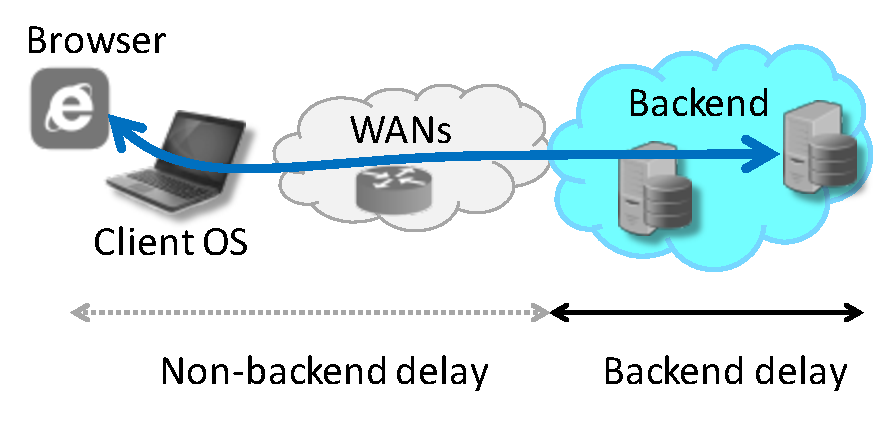
\includegraphics[width=1.0\textwidth]{figs/background.pdf}
%	\caption{\em High-level architecture of web service and the workflow of a web request.}
%	\label{fig:background}
%\end{wrapfigure}
%Figure~\ref{fig:background} depicts the high-level architecture of large-scale web services. %In  typical workflow of a web request.
The end-to-end delay of a web request (\ie page loading time) typically consists of three parts---client-side rendering, wide-area networks (WANs), and the backend system.
%The delay of each component contributes to the end-to-end delay. 
Thus the user-perceived QoE can be affected by the delay of any of these components
(if the requested data is not cached locally by the client/ISP, etc). 
%In today's federated Internet architecture, the web service provider typically only has the control over the backend-induced delay. 
%Note that although client-side browsers/apps are developed by web service providers, the client-side delay is largely decided by how OS share resources among applications. 

A web backend system can be viewed as solving a resource sharing problem: to share limited resources among web requests in order to optimize QoE.
In practice, however, the web service providers only control the backend delay\footnote{Although client-side browsers/apps are developed by web service providers, the client-side processing delay is largely decided by how OS share resources among applications.} and have no direct visibility to the non-backend delay of other systems. 
Consequently, the conventional wisdom has been that the backend system should ensure all requests be processed within a deadline (\eg as described in the service-level agreement~\cite{jang2015silo,serrano2013towards}), under the assumption that other non-backend systems (WANs, browser, etc) would add a random amount of non-backend delay.
%With the web service providers only controlling the backend and the backend-induced delay\footnote{Although client-side browsers/apps are developed by web service providers, the client-side delay is largely decided by how OS share resources among applications.}, they seek to minimize the backend delay. 

\subsection{Our approach: Minimizing the impact of backend delay}

This traditional approach is sensible only if the backend delay has the same effect on any request.
However, {\em the sensitivity of QoE to the backend delay does vary across requests}. %\eg the same 30ms backend delay can affect the QoE of two requests very differently, depending on their non-backend delay.

\begin{wrapfigure}{r}{0.4\linewidth}
	\centering
	\vspace{-0.5cm}
	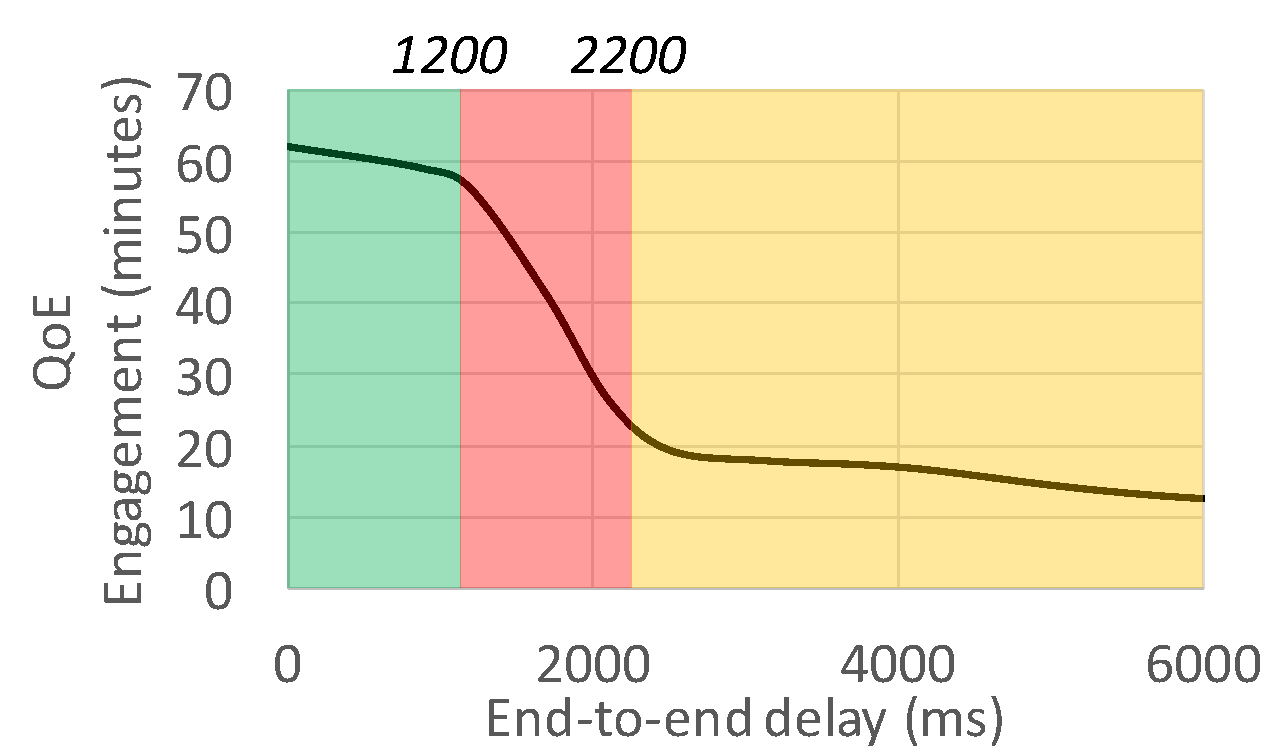
\includegraphics[width=1.0\textwidth]{figs/qoe-curve.pdf}
	\caption{\em QoE curve: relationship between QoE and the end-to-end delay of a request.}
	\label{fig:qoe-curve}
\end{wrapfigure}
\mypara{Key insight: Heterogeneous sensitivity of QoE to backend delay}
To illustrate this observation, Figure~\ref{fig:qoe-curve} shows the {\em QoE curve} (\ie the relationship between QoE and the end-to-end delay of a request) using  a real-world dataset.
%Figure~\ref{fig:qoe-curve} illustrates this using a dataset of \fillme web requests. 
The dataset includes requests to the same page (one of Alexa's top-50 pages) over a span of 24 hours from 12 countries, which represents a decent spatio-temporal coverage of users while avoiding the impact of content-specific factors on QoE.\footnote{The QoE curve may vary with the type of web page (\eg QoE in general is less sensitive to end-to-end delay when the user really needs to see the content of the page), yet the sigmoid-like shape remains~\cite{akamai-report}.} 
%The figure shows the relationship between QoE and the end-to-end delay of a request, which we refer to as the {\em QoE curve}.
%It is based on \fillme requests to a particular page (\fillme), thus avoiding the impact of content on QoE. 
We define QoE of a request by user engagement\footnote{User engagement is one of the standard ways of measuring user experience~\cite{balachandran2014modeling,shafiq2014understanding,dobrian2011understanding}, in part because it is used directly in the click-/conversion-driven revenue models. Similar QoE curve has been observed against other QoE measures (\eg mean opinion score) in the literature too.}---the duration of the user staying on the web page and all subsequent pages linked from the page. 
The end-to-end delay is defined by the page load time~\cite{wang2013demystify}, \ie subtracting when the page is completely loaded from when the request is issued.
The key feature of the QoE curve is its non-linear (sigmoid-like) shape---\ie the impact of the backend delay (\ie small increase of end-to-end delay) on a request's QoE depends on its position on the curve.
It can be explained as following.
Users are not sensitive to an additional backend delay when the overall delay is so short that it is imperceptible or when it is so long that the user has mostly tired of waiting. But when the backend delay is in between these two cases, it can make significant difference. 
In Figure~\ref{fig:qoe-curve}, QoE is much more sensitive to the backend delay when the total delay is between roughly 1200ms and 2200ms than it is below or above that range.


\begin{wrapfigure}{r}{0.4\linewidth}
	\centering
	\vspace{-0.3cm}
	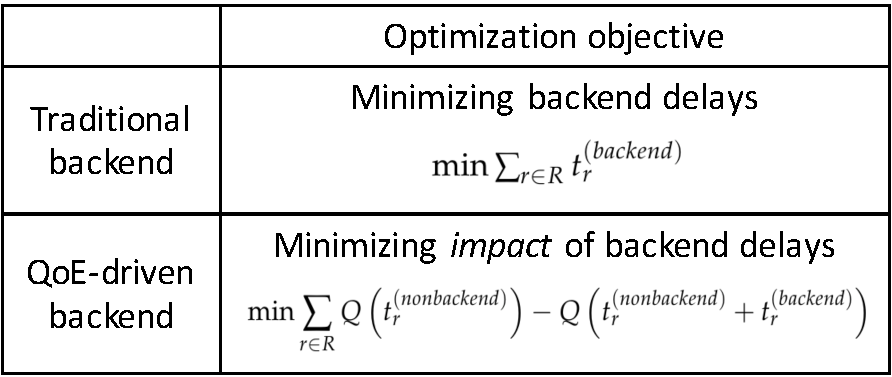
\includegraphics[width=1.0\textwidth]{figs/objective-contrast.pdf}
	\caption{\em Contrasting the traditional control objective with QoE-driven control objective.}
	\label{fig:objective-contrast}
\end{wrapfigure}
\mypara{Changing the optimization objective}
We are not the first to observe such varying impact of backend delay on QoE~\cite{timecard,dqbarge,balachandran2014modeling}, but few prior work has systematically applied this observation to resource allocation in the context of large-scale web services. 
%The control logic needs to be updated too.
Figure~\ref{fig:objective-contrast} illustrates the contrast between the proposed QoE-aware backend and traditional web backend.
Traditional backend seeks to minimize average backend delay of a request set $R$, \ie Eq.~1,
%\begin{align}
%$\min \sum_{r\in R} t_{r}^{(backend)} \label{eq:old}$
%\end{align}
whereas, QoE-aware backend seeks to minimize average degradation of QoE, \ie Eq.~2.
Here, let $t_{r}^{(nonbackend)}$ and $t_{r}^{(backend)}$ denote the non-backend delay and backend delay of a request $r$, respectively, and $Q(t)$ denotes the expected QoE of the total backend and non-backend delay $t$.
%\begin{align}
%$\min \sum_{r\in R} Q\left(t_{r}^{(nonbackend)}\right)-Q\left(t_{r}^{(nonbackend)}+t_{r}^{(backend)}\right) \label{eq:new}$
%\end{align}
%Although ideally, we would like the multiple subsystems of the web backend to jointly optimize the backend delay of each request, there is little support of cross-subsystem orchestration across these subsystems, despite that they are typically owned by the same corporate/organization. So in  the proposed resolution, we only consider making individual subsystems aware of QoE sensitivity. Cross subsystem QoE optimization will be briefly discuss in \S\ref{sec:design}.

\subsection{Motivating scenarios}
\label{subsec:benefits}
%At a high level, rather than treating all requests as having equal sensitivity to the same amount of backend resources, the backend should instead allocate idle resources to requests that are more sensitive to backend delay.
Next, we provide a taxonomy that categorizes the proposed QoE-driven web backend along two dimensions: 
what metrics a QoE-driven backend can improve, and what common backend tasks a QoE-driven backend can improve.

\mypara{Performance metrics that can benefit}
%As the first step, we categorize performance metrics along which a QoE-driven backend outperforms today's backend systems.
\begin{packeditemize}
\item{\em Improving QoE without adding more resources:} 
First and foremost, a QoE-driven backend can achieve better QoE than a traditional one by allocating resources in a way that more explicitly optimizes the total QoE. 
The basic idea is to switch resources from requests that are insensitive to backend delay to those that are sensitive.
We will see an example of this in \S\ref{sec:quantifying}.\footnote{Besides web services, video streaming services can benefit from similar ideas as well. For instance, the video servers can allocate more resources (\eg bandwidth, I/O cycles) to video sessions whose buffer is shallow (\ie the QoE is more sensitive) than to those whose buffer is longer.}
%In contrast to today's web backends which focus on the mean (or percentiles) of backend delay, we argue that they should instead {\em minimize the impact of backend delay on QoE}, so more resources (\eg higher priority) should be given to requests whose QoE is more sensitive to the backend delay. 

\item{\em Saving resources without hurting QoE:}
Similarly, one can reduce resource consumption (and thus save energy) by spending less resources on those requests of lower sensitivity to the backend delay. For instance, this can be done by allocating fewer CPU cycles or memory to servers that serve these requests or sending them to servers with higher load.

\item{\em Mitigating the impact of performance outliers:} 
Web backends are susceptible to performance outliers---excessively long delay due to \eg server garbage collections. 
Rather than trimming the outliers, we take a different approach---reducing the {\em degradation} of QoE caused by outliers.
For instance, we can profile the performance of servers~\cite{yadwadkar2014wrangler}, and assign only requests with less QoE sensitivity to those likely to have outliers. 
    
%\item{\em Cost-efficient explorations:}
%To cope with dynamic resource availability and network conditions, web backends need to monitor the performance of multiple decisions (\eg edge clusters) by sending some random requests to use suboptimal decisions or injecting active probing traffic, neither of which is ideal.
%We take a different approach---we can use the requests that are less sensitive to backend delay to probe the suboptimal decisions, as long as the resulting QoE degradation is below the overall QoE improvement.
\end{packeditemize}
%does not exceed the QoE gain of sending a request of high QoE sensitivity to the optimal decision.
% This way, we can maintain visibility with less impact on QoE.
%\end{packeditemize}
%Note that at first glance, these optimizations may seem unfair, but as we will discuss in \S\ref{sec:arch}, this can still be fair in the sense that each request gets an equal treatment (degradation) on the QoE.

\mypara{Basic backend tasks that can benefit}
%The improvements along performance metrics can manifest themselves in different use cases in web backend (Figure~\ref{fig:framework}): 
\begin{packeditemize}

\item {\em Resource allocation:} 
Better allocation of resources, such as CPU, RAM, network bandwidth, that are shared by multiple concurrent requests. 

\item {\em Scheduling:}
Scheduling of requests shares resources (\eg slots in a queue) along the temporal dimension.
Uses of scheduling include message broker, job scheduler, etc.

\item {\em Replica selection:}
Performance of replicas depends critically on how requests are assigned.
Uses of replica selections include selections of web servers, nodes of a distributed key-value store (or database), partition-aggregating nodes.

\end{packeditemize}
One should note that these benefits can be realized without adding new hardware resources or changing software stack.
% These optimizations might appear unfair at first glance, but fairness can be restored since each request gets an equal treatment, \ie QoE degradation (more on this in \S\ref{sec:fairness}).





\section{Research Plan}

\tightsubsection{Quantifying Potential Benefits in the Wild}
\label{sec:quantifying}
\begin{task}
We will carry out measurement studies to quantify the benefits, in QoE and resource-efficiency, of a QoE-aware web service backend.
\end{task}

%The heterogeneity of QoE sensitivity across requests opens up many new opportunities to strike better resource/QoE tradoffs. 
Before actually implementing and deploying the QoE-driven backend, our first step is to understand how much potential benefit would result from a QoE-driven web backend system in a real-world setting. 
In this section, we outline a measurement study to answer this question in two steps: quantifying the potential performance improvement under the typical workload of a large-scale web backend system, and identifying when exactly the performance would be significant.

%a taxonomy to categorize various possibilities of using the heterogeneous QoE sensitivity to improve the web service backend.%, and show simple-yet-realistic motivating examples to highlight two concrete use cases.


%\subsection{What-if evaluation on the room for improvement}
%\label{subsec:example}
\begin{wrapfigure}{r}{0.55\linewidth}
	\centering
	\vspace{-0.4cm}
	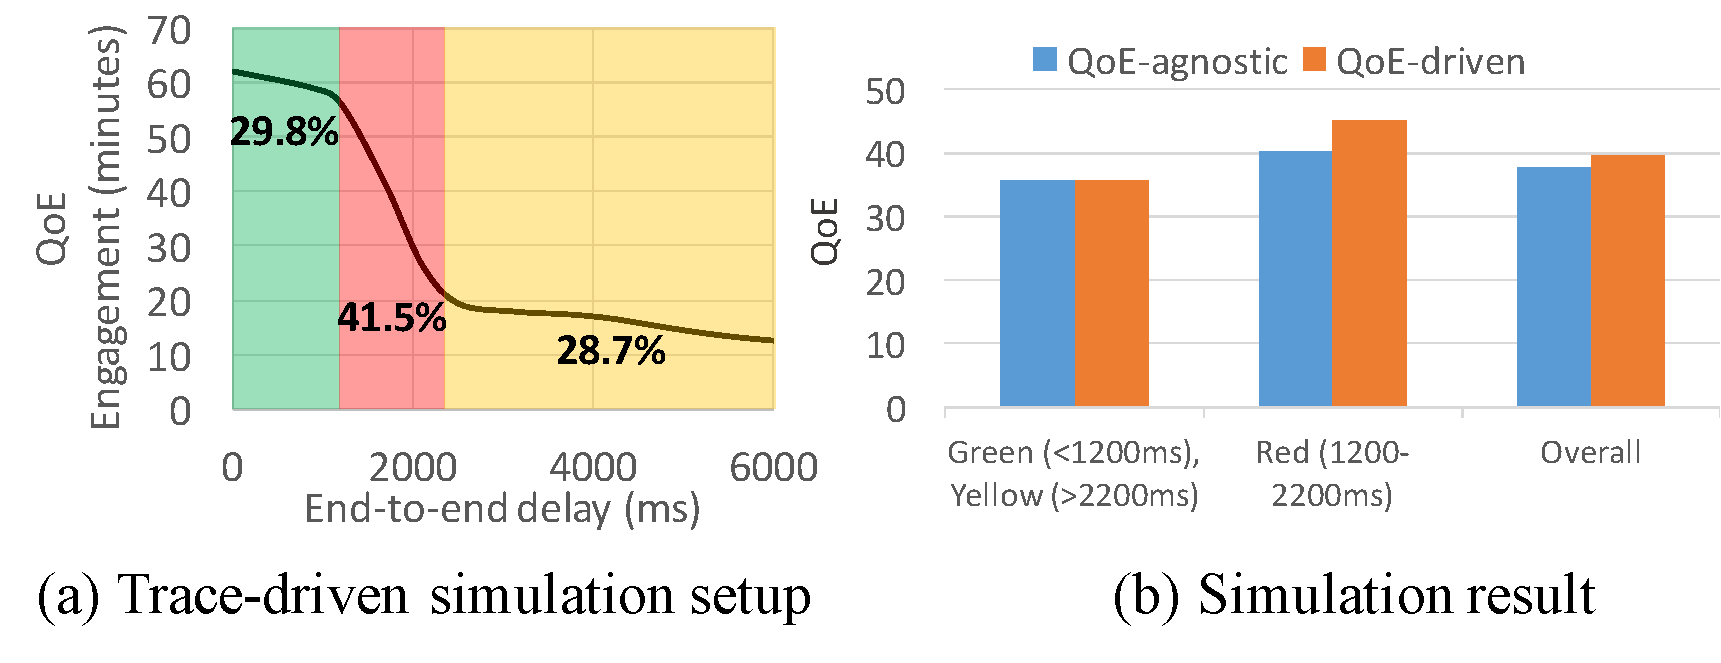
\includegraphics[width=1.0\textwidth]{figs/simulation.pdf}
	\vspace{-1.cm}
	\caption{\em Trace-driven simulation to show QoE improvement}
	\label{fig:simulation}
\end{wrapfigure}
\mypara{What-if evaluation on the room for improvement}
We use a simple trace-driven simulation to illustrate how a QoE-driven backend improves QoE (Figure~\ref{fig:simulation}).
%, and then explain how it differs to traditional resource allocation approaches.
%To see it in action, suppose that request $A$ with non-backend delay $x_a$ is more sensitive to the backend delay (the red area of Figure~\ref{fig:qoe-curve}) than request $B$ with non-backend delay $x_b$ (the green or yellow area of Figure~\ref{fig:qoe-curve}). Now, if the backend resource allocation is such that one of them will get a backend delay of $\delta_1$ and the other one $\delta_2$, $\delta_1>\delta_2$. A QoE-agnostic method may make a random decision (\eg 50\% probability $A$ will get an end-to-end delay of $x_a+\delta_1$), but a QoE-driven method should instead assign the smaller backend delay $\delta_2$ to $A$, because $A$ is more sensitive to backend delay.
%Here, we run a simple simulation to quantify this improvement using the QoE curve shown in Figure~\ref{fig:qoe-curve}. 
Suppose we have 1000 requests whose QoE curve is shown in Figure~\ref{fig:qoe-curve}, and their non-backend delays are such that 29.8\% draw uniformly randomly from 0-1200ms (green part), 41.5\% from 1200-2200ms (red part), and 28.7\% from 2200ms to 6000ms (yellow part). This distribution matches the non-backend distribution in the dataset of Figure~\ref{fig:qoe-curve}.
We pre-generated 1000 backend delay values uniformly between 100-300ms. 
First, we consider a baseline that picks a random backend delay from the 1000 values (without replacement) for each request. The average QoE value is 37.6 minutes (duration spent on the website).
Now, we imagine a QoE-driven policy that assigns the lowest 41.5\% backend delay values to the request between 1200-2200ms, and the rest of the requests get randomly assigned delay values (without replacement). 
The average QoE now is 39.5 minutes, almost two-minute longer than the traditional method. In the QoE of the red part (QoE sensitive users), the improvement is almost 5 minutes longer than the traditional method!
%Note that these improvements could potentially be achieved by simply prioritizing requests differently, without adding new resources or changing the underlying resource allocation mechanism (more on this in \S\ref{sec:design}).
Such improvement may seem small, but improving user engagement by several minutes can make a significant difference for web service providers who use ad-/subscription-driven revenue models.

It is important to note that such outcome will not naturally emerge from traditional methods that assign same resources to each request.
Even traditional deadline-driven policies that prioritize some requests over others (\eg in~\cite{wilson2011better}, a few randomly picked flows might be delayed so that most flows can meet the flow completion deadline), such prioritization is still under the assumption that requests have the same sensitivity to the backend delay.


%\subsection{Understanding the factors affecting improvement}
\mypara{Understanding the factors affecting improvement}
%Next, we examine that under what conditions can QoE-driven web backend significantly outperforms traditional ones. 
This example shows three key factors that affect the magnitude of QoE-driven improvement.
\begin{packeditemize}
\item First, the workload must be a mix of sensitive requests (whose QoE is sensitive to the backend delay) and insensitive ones, as in the previous example.
If all requests in Figure~\ref{fig:qoe-curve} were in the red region, we would see little performance improvement over the baseline, because the backend delay will have the same effect on QoE. 
%The improvement will be significant when sensitive requests and insensitive requests are both present, as in the example of \S\ref{subsec:example}.
%, we found 41.5\% requests have QoE that is sensitive to the backend delay (red region between 1200ms and 2200ms), and the rest (29.8\% in the green region and 28.7\% in the yellow region) have QoE that is not as sensitive to the backend delay. 

\item Second, requests should have different backend delay, which distributed systems naturally have for a number of reasons, \eg jobs in a queue will naturally have different waiting time, or replicas will naturally have different performance since they have different load.

\item Finally, the backend delay must not be too large or small a portion of the end-to-end delay. Too large, the end-to-end delay will be dominated by the backend delay, making all requests similarly sensitive to the backend delay. Too small, the backend delay will only have a very marginal impact on the end-to-end delay and QoE. 
Fortunately, the backend delays typically constitute a non-trivial yet not dominant portion of the end-to-end delay~\cite{dqbarge,mystery,timecard}.
\end{packeditemize}

%\subsection{Proposed research}
\mypara{Proposed research}
%- Quantifying the QoE-delay curve in the wild
We propose to run measurement studies and trace-driven analysis to characterize the QoE-driven opportunities along three aspects.
First, we will perform a mix of user studies and trace-driven analysis to create QoE curve for various web sites (\eg Alexa top sites) and different users (\eg various devices, demographic areas) to confirm that the impact of backend delay on QoE does varies.
%- Quantifying the heterogeneity of QoE sensitivity
Second, we will work with Microsoft, a large web service provider to gain insights on the fraction of backend delay-sensitive web requests in real-world traffic and how dynamic the backend delay of a large-scale web service can be.
Based on our discussion with Microsoft, it is expected that this task can use real-world data.
%- Impact of QoE-aware logic on QoE (maybe delay is too small to be noticed anyway)
Finally, to efficiently explore the whole space of advantages (performance metrics and use cases presented in \S\ref{subsec:benefits}), we plan to scale the evaluation by developing a trace-driven simulator (similar to Figure~\ref{fig:simulation}) that uses real trace to estimate the potential improvement without actually deploying QoE-driven web backend.






\tightsubsection{The Enabler: Estimating Backend's Impact on Per-Request QoE in Real Time}
\label{sec:enabler}
\begin{task}
We will explore new architectural component of web backend, including tracing infrastructure and QoE prediction models, to estimate the QoE sensitivity of requests in real-time.
\end{task}


%\subsection{Framework}
%\label{subsec:framework}
\begin{wrapfigure}{r}{0.4\linewidth}
	\centering
	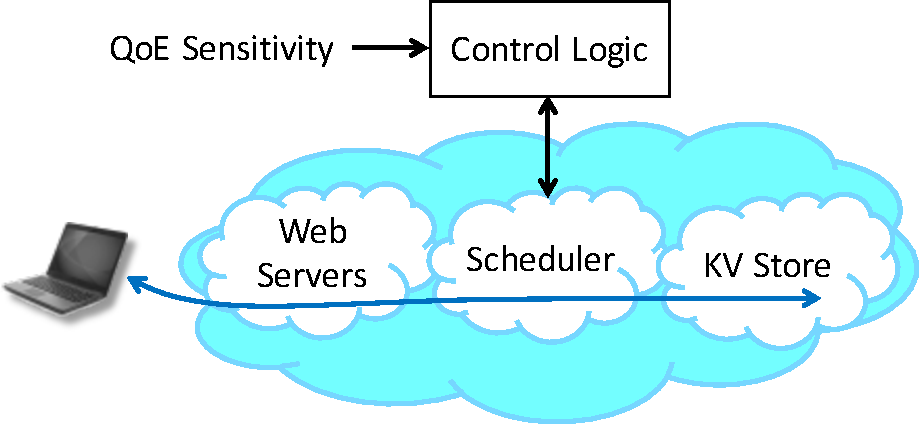
\includegraphics[width=1.0\textwidth]{figs/framework.pdf}
	\caption{\em QoE-driven backend framework.}
	\label{fig:framework}
\end{wrapfigure}
\mypara{QoE-driven backend framework} Figure~\ref{fig:framework} shows the high-level framework of a QoE-driven web backend system.
%Our design takes a pragmatic stance and confine ourselves to the minimal necessary changes on today's web backend.
We envision each individual backend subsystem (web servers, messaging brokers, key-value stores, etc) has a resource-allocation control logic (\eg scheduling, queuing logic, replica selection logic, congestion control), which takes in as part of its input the sensitivity of any request's QoE with respect to the backend delay.
This information can be inferred by estimating its non-backend and finding its position on the QoE curve. 
%We will discuss this in details.
%We envision different ways in which this information would be provided; \eg through a service that predicts the non-backend delay of a new request by profiling the non-backend delay of similar history requests, or adding a field in the request for any subsystem to tag the time it leaves each subsystem. (More discussion in \S\ref{sec:arch}.)


\mypara{Potential approaches to estimating non-backend delay}
Making web backend aware of a request's QoE sensitivity is difficult in today's federated Internet architecture with the web backend system only having the visibility of the delay within its own system, while QoE, defined by either subjective user satisfaction or end-to-end response time, is only observable by the clients themselves. 
We envision that the QoE-delay curve, \ie relationship between end-to-end delay and QoE, should be profiled offline (for each content/application), because it is not expected to change frequently.
If the backend knows the non-backend delay of any incoming request, it would then be able to derive the QoE sensitivity of the request from the QoE-delay curve. 
We envision two basic approaches to measure the non-backend delay of a new request. 
\begin{packeditemize}
\item {\em History-based:}
One can use the non-backend delay of history requests to build a prediction model which, given any new request, can predict its non-backend delay. Once a request is completed, the content provider will know its end-to-end delay (\eg via client-side instrumentation), and by  subtracting the backend delay measured by the backend from the end-to-end delay, we can get the non-backend delay of all history requests.

\item {\em Tracing-based:}
Alternatively, one can directly get the non-backend delay of a request using the tracing infrastructure on the client and backend to directly measure the delay between when the client issues the request and when the backend receives it, \ie the ``incoming half'' of the non-backend delay. Prior work has found that the incoming part of the non-backend delay is indicative of (though not equal to) the ``outgoing'' part~\cite{timecard}.
\end{packeditemize}

% \mypara{What pieces in today's systems can be used}
% In fact, the tracing infrastructure, similar to what is needed for the tracing-based approach, is already available in several large-scale web service infrastructures. Facebook has introduced such a tracing system~\cite{mystery}. Microsoft has a similar internal tracing system that keeps track of several key timestamps of a request (\eg when is issued by client, received by the edge web server, received and processed by a backend database)~\cite{lecuyer2017harvesting,odin}.

%- Cross-subsystem tracing and predicting non-backend delay
In fact, the tracing infrastructure, similar to what is needed for the tracing-based approach, is already available in several large-scale web service infrastructures. Facebook has introduced such a tracing system~\cite{mystery}. Microsoft has a similar internal tracing system that keeps track of several key timestamps of a request (\eg when is issued by client, received by the edge web server, received and processed by a backend database)~\cite{lecuyer2017harvesting,odin}.
% While both history-based and tracking-based approaches sound promising, 

\mypara{Proposed research}
We propose to build tracing and prediction techniques to estimate QoE sensitivity in real time.
While building the system on existing tracing infrastructure sounds promising,
they may not meet the goal of estimating QoE sensitivity of requests in real time. 
These tracing systems and QoE recording systems are mainly built for {\em offline} diagnosis, rather than online inference. As a result, the tracing events are often recorded by individual subsystems in a distributed fashion, but only collected to a central place that can be queried every several minutes or even hours. 
To address this problem requires a better solution. 
Our initial approach would be to make these tracing information (\eg timestamps of the past events of a request) ``in-band'' as part of the request itself. This may require changes in the message format or client-facing interfaces, but will make these tracing information instantly available when the backend receives the request.

Note that the tracing-based and history-based approaches have a tradeoff---the history-based approach requires no additional real-time tracing of a new request and is thus less intrusive to the existing system, whereas the tracing-based approach is more intrusive but might be more accurate as it directly measures the request under consideration.


\tightsubsection{Designing QoE-Driven Control Algorithms}
\label{sec:design}

\begin{task}
We will develop new control policies (including scheduling, replica selection) that leverage the heterogeneity of QoE sensitivity across requests to improve the QoE/resource tradeoffs.
\end{task}

In this task, we will focus on the control logic of scheduling and replica selection as the locus of QoE-driven optimization. 
We start with why traditional scheduling and replica selection policies are insufficient.
Then we highlight technical challenges behind the QoE-driven control logic.

%\subsection{Why are new policies needed?}


%\mypara{Message scheduling}
% - fifo and etc don't work
\begin{wrapfigure}{r}{0.45\linewidth}
	\centering
	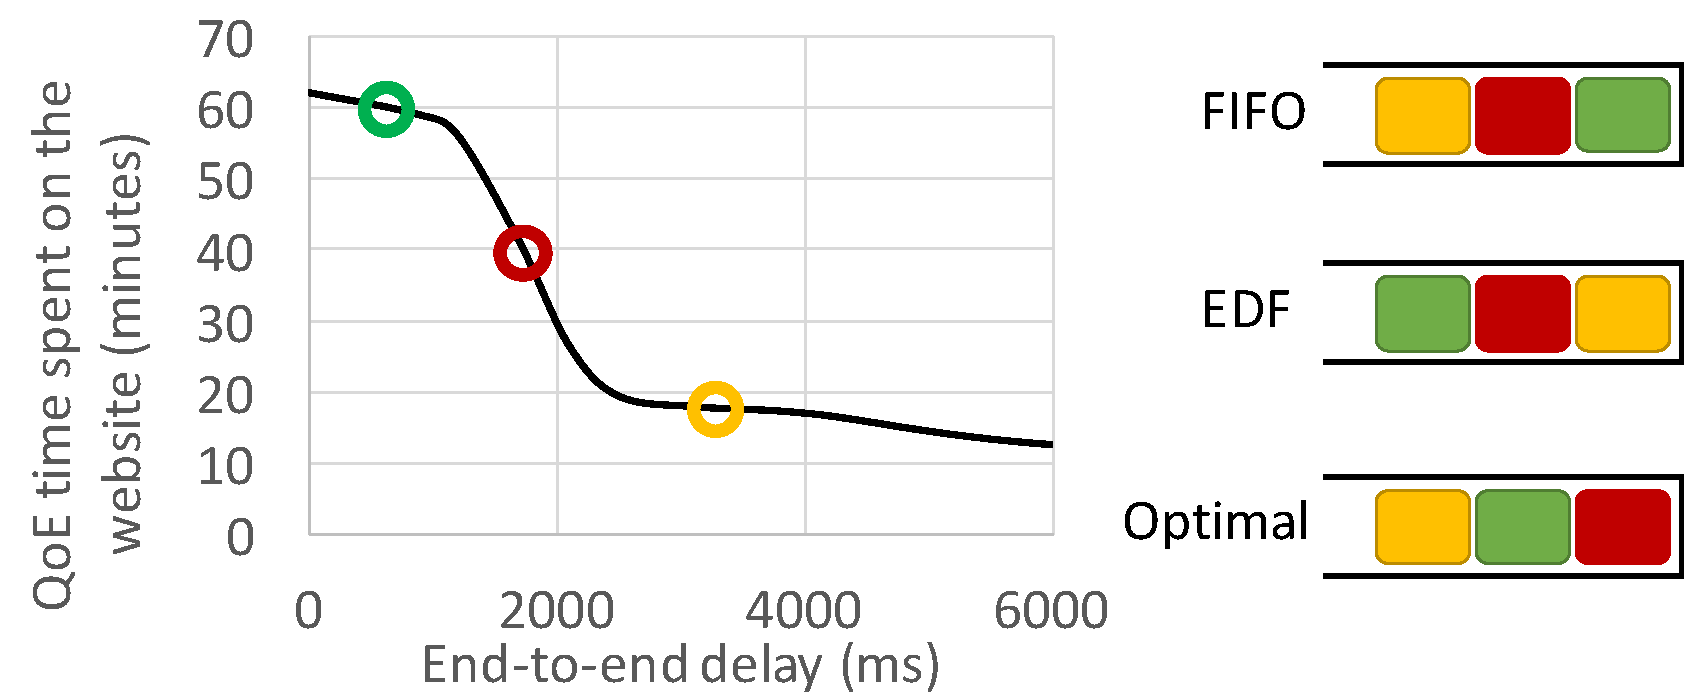
\includegraphics[width=1.0\textwidth]{figs/scheduling.pdf}
	\vspace{-0.6cm}
	\caption{\em The outcomes of different scheduling policies (right) applied on the three requests with different positions on the QoE curve (left).}
	\label{fig:scheduling}
\end{wrapfigure}
\myparaq{Why are new policies needed}
Message scheduling~\cite{rabbitmq,kafka} in queues is pervasively used in the web backend. 
For instance, a message broker is a typical queuing system that provides subscriber/publisher services between two subsystems (\eg web servers and database stores). 
Figure~\ref{fig:scheduling} illustrates the need for a new policy for QoE-driven scheduling. 
We consider three requests in a queue, which are identical except their non-queuing delays (shown on the left-hand side of Figure~\ref{fig:scheduling}).
We compare three policies: 
(1) FIFO, which is the default policy for equal-priority requests.
(2) Earliest-Deadline-First (EDF), which give the requests with longer non-queuing delay higher priority (\ie closer to the deadline), and 
(3) the optimal scheduling policy (Optimal) that maximizes average QoE.
Here, the end-to-end of a request is the sum of the backend delay (\ie the number of jobs ahead of it times the per-request processing delay) and the non-backend delay.
Figure~\ref{fig:scheduling}  shows the outcome of running each policy. 
Because FIFO and EDF are oblivious to the sensitivity of QoE (\ie the slope of each request on the QoE curve), they are not aware that the most sensitive request is the red one.
In contrast, the Optimal policy is able to identify and prioritize the red request one over the others.
%OPT also outperforms EDF with various deadlines, even though it somehow takes the non-queuing delay into account (by imposing a deadline on the total of queuing and non-queuing delay).
%This is because how close a request's non-queuing delay is to the deadline is {\em still} agnostic to the sensitivity of QoE to the queuing delay. 
%Remember in Figure~\ref{fig:qoe-curve}, the QoE sensitivity does not grow monotonically to the non-backenc(queuing) delay. 

%\begin{comment}

%\mypara{Web server replica selection}
% - example of tails
\begin{wrapfigure}{r}{0.5\linewidth}
	\centering
%	\vspace{-0.6cm}
	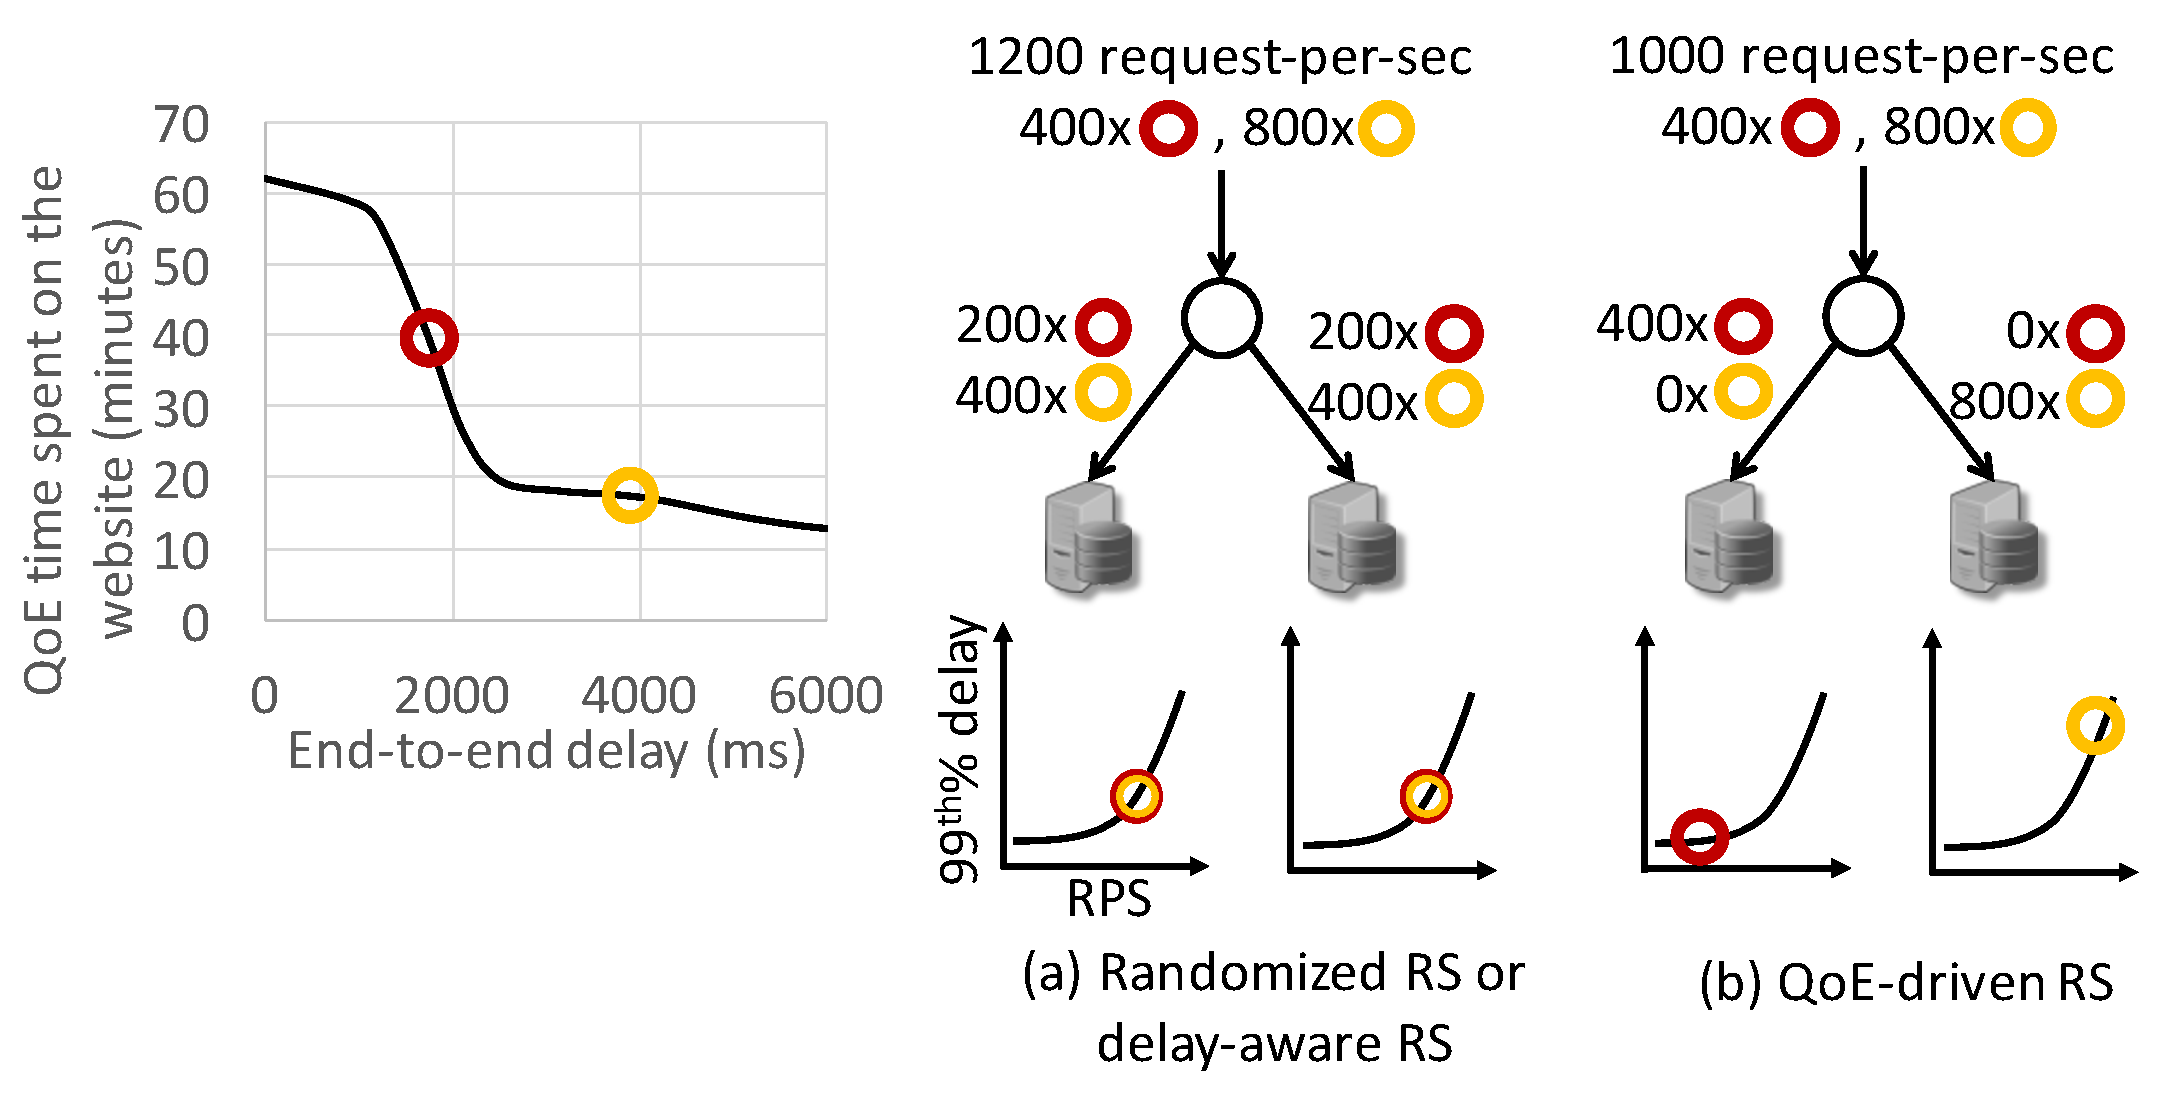
\includegraphics[width=1\textwidth]{figs/replica.pdf}
	\vspace{-0.9cm}
	\caption{\em A simple example showing the outcomes of different replica selection policies.}
	\label{fig:replica}
\end{wrapfigure}
Another example where today's control logic is insufficient is replica selection in distributed database (\eg~\cite{cassandra}).
Large-scale distributed systems are susceptible to {\em performance outliers}.
% on some replicas---\eg exceptionally long processing time on some requests due to CPU contention, software garbege collection, etc. 
Despite much effort to eliminate performance outliers, they are still prevalent, resulting in bad tail (\eg 99$^\textrm{th}$ percentile) performance even if the mean/median performance is good.
%Our first idea is that rather than cutting the performance outliers, we show that QoE-aware replica selection algorithm can {\em contain} the negative impact of performance outliers on user-perceived QoE.
%Consider a system with two replicas, as in Figure~\ref{??}. 
Figure~\ref{fig:replica} illustrates an example where a QoE-driven replica selection policy can contain the negative impact of performance outliers on user-perceived QoE, but a traditional load-balancing policy is not able to do so.
Both replicas have the same load-performance profile: as load (number of requests received per second) goes up, the 99$^\textrm{th}$ percentile delay increases sharply. We assume that the mean delay remains the same. 
This illustrative setting is simplified but is consistent with the load-performance profile in real datacenters. %~\cite{??}.
Suppose that the workload is 1200 requests per second, that the requests have same QoE curve, and their non-backend delays follow the distribution show in the figure.
We compare two traditional replica selection policies---a randomized policy that strives to put even load, a latency-aware policy (\eg~\cite{suresh2015c3,wu2015costlo}) that minimizes average response time---with a QoE-driven policy that minimizes the impact of the processing time on QoE.
The optimal solution achieves better tail QoE than both baselines. 
Both load balancing policy and latency-aware put even load on the replicas, which make both equally overloaded, causing long tail delay and bad tail QoE.
In contrast, the optimal policy diliberately puts more requests on one than another, but does so by letting QoE-sensitive requests use the lighter-loaded replica and letting QoE-insensitive requests use the slightly more loaded replica. 

% In short, we see that, in both scheduling and replica selection, traditional QoE-agnostic policies are fundamentally unable to achieve the same performance as optimal QoE-driven policies. However, implementing an optimal  QoE-driven policy in practice is challenging.


%\end{comment}


\myparaq{Why it is challenging}
In general, a QoE driven policy should meet two requirements: {\em near-optimal} (\ie achieve QoE close to the optimal scheduling outcomes) and {\em efficient} (\ie constant decision time on each incoming request).
To see why meeting both requirements is challenging, let us take scheduling as an example and consider two baselines.
%The new QoE-aware scheduling policy should be {\em near optimal} (\ie achieve QoE close to the optimal scheduling outcomes) and {\em efficient} (\ie constant decision time on each incoming request).
%To see why it is challenging to meet both requirements simultaneously, let us consider two baselines.

On one hand, our problem is non-convex (Figure~\ref{fig:objective-contrast}), so standard approximating
%\footnote{Unfortunately, optimizing a non-convex curve objective function, as in our case, requires running complex algorithms, whose runtime increases super-linearly with the number of variables.}
algorithms (\eg~\cite{udell2013maximizing}) often requires non-constant overhead to compute the scheduling order of each request. 
On the other hand, fast scheduling algorithms can be suboptimal. 
For instance, one efficient scheduling algorithm is to give each request a priority that is proportional to the {\em slope} of its non-queuing delay on the QoE-delay curve. 
This makes sense, because if the request were to stay in the queue for a (short) fixed amount of queuing delay, this slop indicates exactly how much QoE degradation will be caused by the queuing delay, and the decision runtime is constant for each request.
However, the queuing delay does vary among requests as well as over time (as it might be pre-emptived by future requests), and the resulting QoE might suffer.
If the queuing delay is non-trivial, the slope of a request's non-queuing delay can be both an overestimate or underestimate of the actual QoE sensitivity of a request. 
In Figure~\ref{fig:qoe-curve}, for instance, if the queuing delay is 200ms, a request with 1100ms non-queuing delay will be believed as insensitive to the queuing delay, while after 200ms queuing, it actually will see significant drop in QoE. 

%\begin{comment}

Moreover, the new scheduling policy has to be {\em amenable} to the implementation of existing message brokers. 
Take RabbitMQ as a canonical example. 
Logically, it maintains a number (at most 255) of queues, the queues have different priorities, and within each queue, the messages, or requests in our contenxt, are scheduled using simple First-In-First-Out policy (FIFO) policy.
So once a request is pushed to a FIFO queue associated with some priority, and cannot be easily changed to another FIFO queue. 
That means, the related ordering of two requests cannot be changed once they are scheduled.
For instance, the aforementioned slope-based scheduling algorithm cannot be easily fixed by re-assigning a priority that reflects the slope after the amount of queuing delay.
(Note this does not preclude the possibility of preemption by a future request with a high priority.)

%\end{comment}

%Here, the backend delay means the queuing delay (amount of time a request stay in the queue), and the non-backend delay means any delay that is not caused by queuing.

%\jc{cross subsystem optimization}

\mypara{Proposed research}
We propose to develop new scheduling and replica selection policies that leverage the heterogeneity of QoE sensitivity across requests to improve user-perceived QoE while saving resources. 
One potential idea is to rely on the fact that the number of requests and the distribution of their non-backend delay is relatively stable at a timescale of several seconds, so we can {\em predict} the workload for the next few seconds.
Thus, we can periodically recalculate the scheduling (or replica selection) decision for requests of any non-backend delay by assuming that future requests will be drawn from the predicted distribution.
We save this mapping in a look-up table, and when a new request arrives, we can determine the scheduling priority or selected replica for the new request by looking up the table.

Finally, as an extension of making individual subsystems QoE-driven, we will also examine possibilities of joint optimization across subsystems. The problem will become more challenging and will call for more complex solutions, but we believe the insights (\eg persistent workload) from single subsystem control policy may apply to a cross-subsystem setting.





%\newpage 






\section{Putting It into Perspective}
Here we contrast our proposal to three categories of closely related prior work.

\mypara{Improving quality-latency tradeoffs for web services}
That the impact of web backend varies across users has been observed and used before. 
Timecard~\cite{timecard} allows requests with lower network delay to wait longer for the web server to retrieve better ad content. 
DQBarge~\cite{dqbarge} similarly trades delay for better response quality by monitoring the progress of parallel subtasks and allowing non-critical-path subtasks to be process longer to get better results without increasing the total response time.
Driven by the same need to cope with the spatial/temporal heterogeneity of network conditions across users, some works (\eg~\cite{jayathilaka2015response}) try to predict the response-time service-level agreement of cloud applications.
% Also relevant are works that dynamically predict the response-time service-level agreement of cloud applications~\cite{jayathilaka2015response}, which are driven by the same need to cope with the heterogeneity of non-backend delay across users and over time.
Web page prioritization techniques (\eg~\cite{butkiewicz2015klotski,netravali2016polaris}) try to re-schedule the loading of web objects in order to maximize perceived quality.
Closest to this proposal is our prior work EONA~\cite{eona}, which pioneers the idea of driving individual systems (including web service backend) by user-perceived QoE.
However, none of these works leverages the heterogeneity of users' tolerance of backend delay through the lens of resource/QoE tradeoffs. 

\mypara{Application-aware cloud scheduling}
Jointly optimizing application-level objectives with network- or system-level mechanisms is a heavily studied topic. 
Deadline-driven scheduling and congestion control~\cite{vamanan2012deadline,wilson2011better} seeks to finish as many flows as possible by dynamically prioritizing flows with closest deadlines.
Coflow and its variants~\cite{coflow,chowdhury2015efficient} shows that by grouping network flows that are previously treated independently, application-aware network scheduling can significantly improve the cloud application performance.
However, these works assume the applications run within the scope of cloud, and fail to leverage the heterogeneous impact non-cloud factors have on the application performance.

\mypara{Video QoE-aware network management}
It is well-known that user-perceived QoE is different from system-level quality of service (QoS) metrics. 
The most relevant works based on this insight are those that manage network resources to maintain multimedia QoE at desirable level~\cite{barakovic2013survey,hobfeld2012challenges,seufert2015survey,joseph2014nova}. 
For instance, a QoE-aware network controller uses estimate user-perceived video QoE~\cite{huysegems2012session} to improve the video streaming via traffic shaping~\cite{petrangeli2015network} so that minimal storage and network resources are allocated to maintain a specific level of user satisfaction.
However, these works do not consider that some users may be bottlenecked by other systems (other ISPs, CDNs, or home network), and thus fail to take into account users whose QoE might be made desirable by more network resources as well as users whose QoE requirement cannot be met.




\section{Project Scheduling and Plan}

The project will be carried out by the PI and one Ph.D. student who is very familiar with the topic, over a 2-year period.
Though three tasks sound like a lot, they have overlaps (\eg Task 2 can re-use the data collection platform in Task 1) and the systems can be built on top of existing software or platforms (\eg Task 3 can be built by only modifying open-source software like Apache Kafka or Cassandra), which makes it feasible to finish in a span of 2 years.
The timeline is shown below (R=research, B=system building, U=user study \& data collection, E=evaluation).
\begin{table}[h]
\footnotesize
\begin{tabular}{|l|l|l|l|l|l|l|l|l|}
\hline
Research tasks                           & Y1Q1 & Y1Q2 & Y1Q3 & Y1Q4 & Y2Q1 & Y2Q2 & Y2Q3 & Y2Q4 \\ \hline
Task 1: Quantifying potential benefits   & U    & U/R  & U/R  & U/R  &  R    &  R    &      &      \\ 
Task 2: Estimating QoE sensitivity &      & R    & R  & R/B  & R/B    & B/E    & E    & E    \\ 
Task 3: QoE-driven control algorithms    &    &   R    & R  & R/B  & R/B  & B/E  & E   &  E   \\ \hline
%Task 4: Impact on QoE fairness           &      &      & U/R  & U/R  & R    & R    & E    & E    \\ \hline
\end{tabular}
\end{table}






































